\def\DevnagVersion{2.15}%% report.tex
%% V1.0
%% 2013/03/30
%% by Prashant Jalan
%% See:
%% www.prashantjalan.com
%% for current contact information.
%%
%% This is a report file for the semester project I did during my fourth 
%% semester under Prof. Amitabha Mukerjee. The word deals with noun 
%% recognition through a syllablic semantic approach for grounded videos

\documentclass[12pt, a4paper]{report}
\usepackage[left=1.0 in, right=1.0 in, top=1.0 in, bottom=1.0 in]{geometry}

% *** URL PACKAGE ***
\usepackage{hyperref}
% *** HINDI PACKAGE ***
\usepackage{devanagari}
% *** CITATATION PACKAGE ***
\usepackage{cite}
% *** GRAPHICS RELATED PACKAGES ***
\usepackage{graphicx}
% *** MATH PACKAGES ***
\usepackage[cmex10]{amsmath}
% *** ALIGNMENT PACKAGES ***
\usepackage{tabularx}
\usepackage{array}
\usepackage{mdwmath}
\usepackage{mdwtab}
\usepackage{eqparbox}

\begin{document}
\title{Syllable based noun recognition\\for grounded videos}
\author{Prashant Jalan
\\Department of Computer Science \& Engineering\\
Indian Institute of Technology Kanpur\\
Homepage: www.prashantjalan.com}

\maketitle
\tableofcontents

\renewcommand{\abstractname}{Acknowledgements}
\begin{abstract}
I would like to thank Dr. Amitabha Mukerjee under whose supervision I did this work. If not for his guidance, motivation and support, this work would not have been possible. I am thankful that he gave me an opportunity to work under him.\\
\\
I am thankful to Mr. Diwakar Chauhan who was always there to help me understand the difficult concepts and motivate me throughout the project.\\
\\
I acknowledge the excellent word of Nikhil Joshi\cite{nikhil} in 'unsupervised language learning for complex 3D videos'.\\
\\
I owe to my parents and my sister for their moral support and encouragement.\\
\\
Finally, I thank IIT Kanpur for giving me this platform to pursue my interests and do this research work.



\end{abstract}

\renewcommand{\abstractname}{Abstract}
\begin{abstract}
We aim to make the computers learn a new language without any previous knowledge about the language. In this work, we have used a semantic syllabic approach and also a word level analysis to acquire basic linguistic units particularly, noun based on the Langacker\cite{langacker} theory of learning language. Based on a 2D video and co-occurring raw text, we demonstrate how this cognitively inspired model segments the world to obtain a meaning space, and combines words into hierarchical patterns for a linguistic pattern space. We try to recognize nouns in the English language and the Hindi language based on some narrations taken from different subjects using different association measures such as the mutual information, relative frequency and conditional probability.
\end{abstract}


\chapter{Introduction}
\section{Language learning framework}
The problem of language acquisition has been of great interest to many disciplines including Linguistics, Psychology, Philosophy, Neurobiology, Cognitive science and Computer Science. From Panini\cite{panini} to Chomsky\cite{chomsky} to Tomasello, there have been many attempts to formalize the theory of language. The debate is mostly two-sided. Chomsky\cite{chomsky} argues for the innateness of language based on the argument (known as `poverty of stimulus') that the child acquiring language has access to only positive examples (grammatical sentences), and very little corrective feedback. Thus, the Chomskyan framework focuses on the syntax of a language and is largely sceptical about semantics. So, learning a language from his viewpoint is learning a `generative syntax' for that language. Langacker\cite{langacker}, alternatively has given a central role to semantics in his language learning model. Langacker\cite{langacker} considers grammar as conceptualization and formalizes it as a bipolar symbolic unit interconnecting the phonological pole (linguistic representation) and the semantic pole (conceptual representation). In the view of cognitive grammar, language is entrenched in the usage and linguistic representations get their meanings because of their usage with some conceptual entity.
The idea is analogous to a child’s way of learning. When a child is born, he knows nothing about a language. He doesn’t know anything about the noun, verb, preposition or the syntax or the word boundaries. But as he continuously hears description, slowly after many instances of a particular object or an action been referred to by a particular word, the child begins to recognize the word and associate it with the object or action. 

\section{Resources exploited}
We used python as the programming language because of its ability to handle large datasets and execute complex algorithms with very simple commands. We used Windows Movie Maker to record narration for the video clips and export it without any change in the video properties such as the frame number, bit rate and frame size. We had also used the VideoPad Video Editor software to embed the audio clip (recorded using the Windows default sound recorder software) onto the video clip. We used Microsoft Word or Open Office to manually transcribe the audio into written Hindi text. To write in Hindi we also used the online editor available at \cite{quill}. 

\chapter{Collecting the dataset}

We collected our dataset by asking different subjects from different linguistic backgrounds to describe the objects and their actions as they saw in the 2-D grounded video.

\section{Collecting Narrations}

We collected narrations in Hindi from twenty one different subjects. Out of them ten subjects had the words {\dn lAl} and {\dn nFlA} in their narrations and eleven subjects had the words {\dn CoVA} and {\dn bwA} in their narrations. For English, we collected narrations from thirteen subjects. Ten subjects used the words \textbf{big} and \textbf{small} and five used \textbf{red} and \textbf{blue} in their narrations.\\
\\
Each subject was given the same set of instruction, the instruction set being `You will be shown this 39 seconds video thrice. For the first two times you can just see the video and gain an understanding of what is happening in the scene. The third time you have to describe whatever is going on in the video in Hindi/English without involving yourself in the description. You are also not allowed to metaphorize the objects in the video.' \\
\\
The subject couldn’t involve themselves in the narration as then the narration would not be just describing two simple objects and their actions in the grounded video, rather it would become a more complex set of narration involving the objects and their actions in the video, the narrator and his actions during the narration.\\
\\
Another crucial phenomenon we observed while taking narrations was the occurrence of an inadvertent time lag between the action going on in the video and the words describing it. This time lag varied from person to person and could be positive. The purpose of showing the video thrice was to reduce the time lag.\\
\\
The speaker were also asked not to metaphorize the objects in the video when we found some speakers replacing the object with some other noun, for instance {\dn CoVA E/\7{B}j} with {\dn cor} and {\dn bwA E/\7{B}j} with {\dn \7{p}Els}.

\section{Audio to text transcription}

Since, the audio speech recognition for Hindi is not yet very efficient and as our primary aim is learning language, we manually transcribed the audio clips into written Hindi texts. While transcribing the utterances, every two consecutive words were separated by space to maintain word boundary. The post-positions were generally treated as separate words and hence were separated from the content words they were attached to. However, the morphological variations were preserved and transcribed as it is without separating them from their roots. While transcribing small grammatical corrections were made. The care was taken to follow uniform writing style to avoid the transliteration variations. We embedded the narration with a reference to the frame number and broke it whenever then was a pause or any sound not describing a proper Hindi word (breathing sound or any other sound due to an external stimulus). If any pause was more than five frames, we made a separate row stating the frame period and entered empty text(nothing). For less than five frames we would merge the pause in the starting of the next narrative sentence as it was not possible manually to achieve an accuracy of less than five frames pause.

\begin{figure}[!t]
\centering
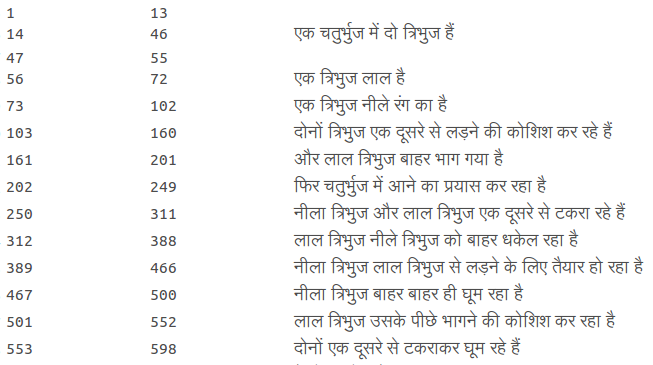
\includegraphics[width=5in]{HN.png}
\caption{\small \sl A narration in Hindi.}
\label{fig_FSM}
\end{figure}

\begin{figure}[!t]
\centering
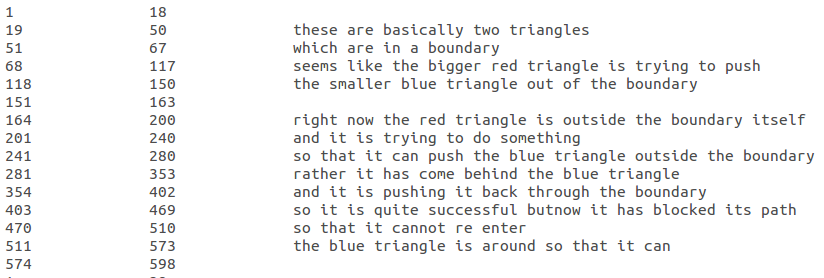
\includegraphics[width=5in]{EN.png}
\caption{\small \sl A narration in English.}
\label{fig_FSM}
\end{figure}

\chapter{Learning the language labels}
This chapter describes the theoretical concepts behind the noun recognition. We experiment with various kinds of linguistic units, different association measures and different datasets. Typically, we assume the linguistic units to be contiguous (k-grams) at word and syllabic-level. We also experiment with units of different lengths combined to form phrases at word and syllabic level. We propose a mechanism to learn the appropriate units of correct size based on fragment analysis and unit-independence conjecture.

\section{Attention Model}
We use an attention model to find the most salient part of the scene. Such a model tries to predict the part of the scene the human is most likely to attend to. The words used in the description are more likely to refer to objects that are in perceptual focus, i.e. we assume that linguistic focus follows perceptual focus.\\
\\
Our attention model is based on the findings that objects that are moving are likely to be more salient. We ignore some other factors such as color and texture, which are more relevant in still images; for image sequences, motion and size are more significant. Size and speed are also not a major factor is our attention model as the objects are not always moving together. For appreciable amount of time in the video, we find that when one object is moving the other isn’t and therefore, the perpetual focus will mostly be guided by the moving object.

\section{Linguistic segmentation}
Linguistic segmentation refers to breaking down the utterances into smaller linguistic units. However, what the smaller linguistic unit of break-up should be is a debatable issue. In our syllabic analysis, we broke the text into syllables without any knowledge of the word boundaries and in our word analysis, we took a single word as one linguistic unit.\\
\\
A unit of pronunciation having one vowel sound, with or without surrounding consonants, forming the whole or a part of a word is defined as a syllable. We have used the following FSM (Finite State Machine) to formulate an algorithm to find the syllabic units from the text assuming that we don’t know the word boundaries.\\
\\
In the FSM, \{C\}, \{V\}, \{M\}, \{O\}, \{P\}, \{S\}, \{H\}, \{D\} denotes the set of all consonants ({\dn k}, {\dn K}, {\dn g},...), vowels ({\dn a}, {\dn aA}, {\dn i}, {\dn I}, ...), matras ({\dn kA}, {\dn kF}, ...), accompanying consonants in Hindi, the character {\dn :}, punctuation marks ({\dn .}, {\dn ..}, ...), signs ( {\dn \2}, {\dn ,}, {\dn \1}, ...), halant and the digits in the Hindi language respectively. The program starts from the $initial$ state. In the $store$ state whatever has been pulled out from the text list is stored as a syllable and in the $ignore$ state it is ignored. From the $initial$ state the machine goes to the $ignore$, $store$, $consonant$ or $vowel$ state depending on what it scans out of the list of text. Similarly, it proceeds forwards from the $consonant$ and $vowel$ state.

\begin{figure}[!t]
\centering
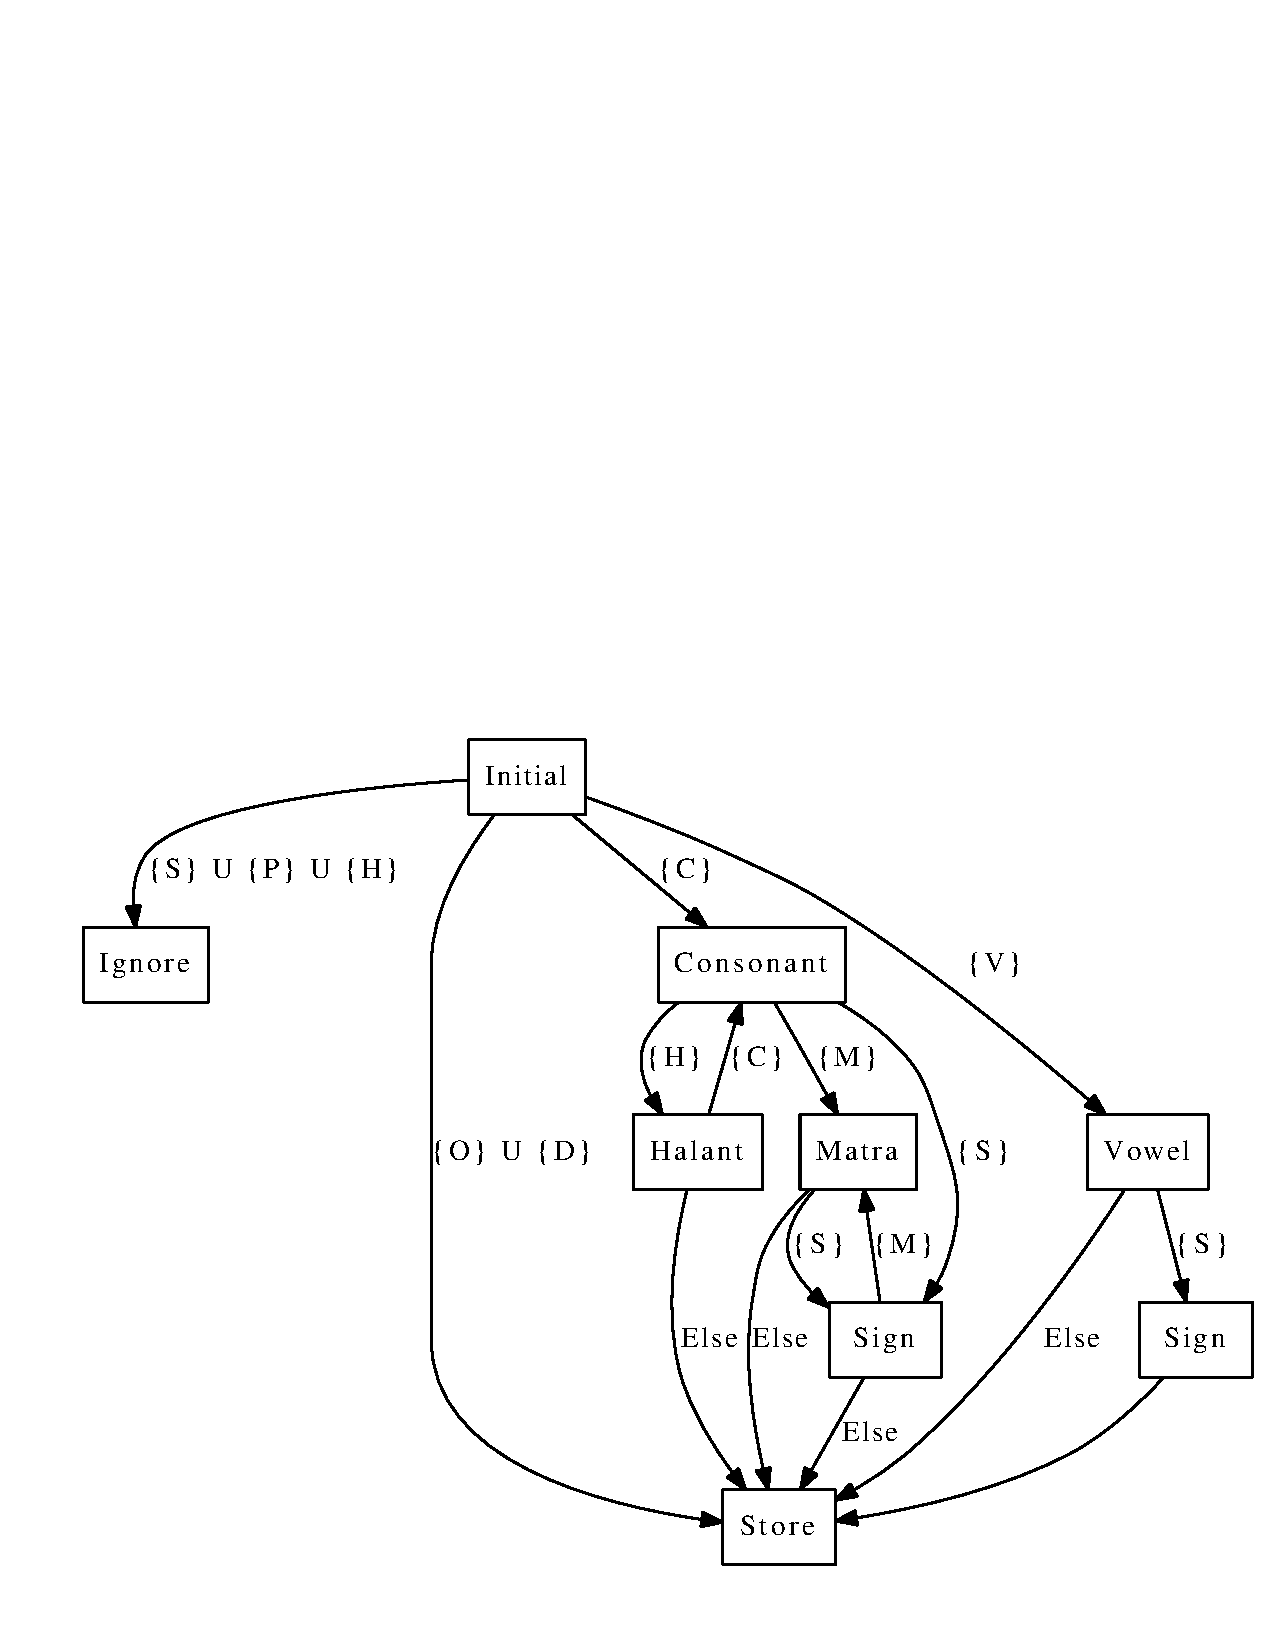
\includegraphics[width=5in]{FSM.pdf}
\caption{\small \sl FSM to identify the syllables.}
\label{fig_FSM}
\end{figure}

\section{Label Association}
For a label $l$, concept $c$, speaker $s$ and time $t$, we define following probabilities.\\
\\
Attention probability of the concept $c$ for the speaker $s$ at time $t$\\
$$
P(c|s,t) = \begin{cases} 1 & \mbox{if $c$ is attended by speaker $s$ at time $t$} \\ 0 & \mbox{otherwise}\end{cases}
$$
\\
$$
P(l|s,t) = \begin{cases} 1 & \mbox{if $l$ is uttered by speaker $s$ at time $t$} \\ 0 & \mbox{otherwise}\end{cases}
$$
\\
We define the Joint probability of a label $l$ and an object category $c$ as\\
$$
J(l|s) = \frac{1}{T \ast |S|} \ast \sum_{t=1}^{T}\sum_{s \in S}P(c|s,t) \ast P(l|s,t) 
$$
\\
Similarly, we define the concept probability of a concept $c$ as\\
$$
P(c) = \frac{1}{T \ast |S|} \ast \sum_{t=1}^{T}\sum_{s \in S}P(c|s,t)
$$
\\
The label probability of a label $l$ is given as\\
$$
P(l) = \frac{f(l)}{\sum_{l}{f(l)}}
$$
\\
where $f(l)$ is the frequency (number of occurrences) of label $l$ in the narrative corpus.


\section{Association Measure}
To find the maximally associated linguistic unit for a given visual category, we need an association measure which can rank the labels according to the degree of co-occurrence between the label and the visual category. A typical association measure should have following properties:\\
\begin{itemize}
\item It should give high association values if the label and the visual category co-occur frequently.
\item It should penalize the labels which co-occur frequently with many categories whereas should prefer labels which co-occur frequently only with a particular category.
\end{itemize}
Various association measures we experimented with are described next.

\subsection{Conditional Probability}
Conditional probability of a label $l$ given a concept $c$ is given as\\
$$
P (l|c) = J(l, c)/P (c)
$$
\\
Conditional probability of a label given concept favours the concepts having rare occurrence but having sufficient co-occurrence with the label. However, it doesn’t consider the distribution of the joint probability of the label over all concepts and hence fails to capture the second property of association measure.

\subsection{Mutual Information}
Mutual information of a label $l$ and a concept $c$ is given as\\
$$
MI(l, c) = J(l, c) \ast log(\frac{J(l, c)}{P (c) \ast P (l)})
$$
\\
Mutual information favours the rare concepts and rare labels having sufficient degree of co-occurrence.

\subsection{Relative Frequency}
Relative frequency of a label $l$ and a concept $c$ is given as\\
$$
P(c|l) = \frac{P(l|c) \ast P(c)}{P(l)} \propto \frac{P(l|c)}{P(l)} \propto \frac{\text{freq ($l$) when c is happening}}{\text{freq ($l$)}} = relative frequency
$$
\\
Relative frequency is therefore a measure of the conditional probability that a concept $c$ has occured given that the label $l$ is uttered.

\section{Other adjustments}

We also experimented by making small changes to obtain better results. We wrote a \textit{shift\_frame} function which would shift the frame record of a concept by the specified amount of frames. This was incorporated to deal with the inadvertent time lag. We removed the k-grams having very less frequency (occurred only once) to minimise their negative impact on the result through a function called \textit{ignore\_freq}. We also wrote a function called \textit{morphology} which removed only specific word inflections, for instance, \textbf{bigger} was made \textbf{big}, {\dn nFl\?} to {\dn nFlA}, etc. Function \textit{merge\_common} merged the frequency of smaller k-grams with that of the bigger k-gram if both had the same frequency and if the smaller k-gram was a sub-string of the bigger k-gram.

\chapter{Corpus Analysis}
While learning the linguistic units, we did not consider the most common and frequent words used in English and Hindi. For English, we took the most commonly used words from a previously done analysis using British English Corpus, American English Corpus and recorded talks and speech\cite{eng-corpus}. For Hindi, we use Hindi unicode corpus, Center For Indian Language Technology, IIT Bombay\cite{hindi-corpus}. We perform both syllabic and word analysis in the Hindi corpus to discover the most frequent words and top k-grams in Hindi. Files with detailed data can be found at \cite{corpus-result}

\section{Most frequent words in Hindi}
The most frequently used words in Hindi are as follows:\\
\\
\begin{tabularx}{\textwidth}{l|X|l|X|l|X|l|X|l|X}
1 & {\dn k\?} & 11 & {\dn BF} & 21 & {\dn is} & 31 & {\dn T\?} & 41 & {\dn jA}\\
2 & {\dn h\4} & 12 & {\dn nhF{\qva}} & 22 & {\dn Ele} & 32 & {\dn TF} & 42 & {\dn rhA}\\
3 & {\dn m\?{\qva}} & 13 & {\dn Ek} & 23 & {\dn kr} & 33 & {\dn n} & 43 & {\dn m\4{\qva}}\\
4 & {\dn kF} & 14 & {\dn ek} & 24 & {\dn vh} & 34 & {\dn \7{k}C} & 44 & {\dn koI}\\
5 & {\dn s\?} & 15 & {\dn hF} & 25 & {\dn EkyA} & 35 & {\dn jAtA} & 45 & {\dn v\?}\\
6 & {\dn aOr} & 16 & {\dn ho} & 26 & {\dn gyA} & 36 & {\dn sAT} & 46 & {\dn \7{h}e}\\
7 & {\dn kA} & 17 & {\dn to} & 27 & {\dn tTA} & 37 & {\dn yA} & 47 & {\dn !p}\\
8 & {\dn ko} & 18 & {\dn yh} & 28 & {\dn krn\?} & 38 & {\dn tk} & 48 & {\dn EksF}\\
9 & {\dn h\4{\qva}} & 19 & {\dn TA} & 29 & {\dn jo} & 39 & {\dn hotA} & 49 & {\dn \7{h}aA}\\
10 & {\dn pr} & 20 & {\dn n\?} & 30 & {\dn apn\?} & 40 & {\dn EdyA} & 50 & {\dn us\?}\\
\end{tabularx}
      
\newpage        
\section{Top k-grams in Hindi}
The top 2,3,4,5,6 k-grams in Hindi are as follows:\\
\\
\begin{tabularx}{\textwidth}{ |X|X|X|X|X|X }
\textbf{2-gram} & \textbf{3-gram} & \textbf{4-gram} & \textbf{5-gram} & \textbf{6-gram}\\
\vspace{5px} & \vspace{5px} & \vspace{5px} & \vspace{5px} & \vspace{5px}\\
{\dn kr} & {\dn k\?Ele} & {\dn n\?k\?Ele} & {\dn krn\?k\?Ele} & {\dn krn\?k\?Ele}\\
{\dn aOr} & {\dn krn\?} & {\dn krn\?k\?} & {\dn rn\?k\?Ele} & {\dn yAjAsktAh\4}\\
{\dn pr} & {\dn apn\?} & {\dn sktAh\4} & {\dn is\3FEwkAr} & {\dn k\?aADArpr}\\
{\dn is} & {\dn n\?k\?Ele} & {\dn EkyAgyA} & {\dn k\?a\7{n}sAr} & {\dn kFaAv\35BwyktA}\\
{\dn tAh\4} & {\dn jAtAh\4} & {\dn aAv\35Bwyk} & {\dn aAv\35BwyktA} & {\dn EkyAjAsktA}\\
{\dn ek} & {\dn h\4aOr} & {\dn srkAr} & {\dn jAsktAh\4} & {\dn algAlg}\\
{\dn nhF{\qva}} & {\dn yAgyA} & {\dn k\?kArZ} & {\dn EkyAgyAh\4} & {\dn u\381wr\3FEwd\?f}\\
{\dn us} & {\dn h\4is} & {\dn rn\?k\?El} & {\dn yAjAsktA} & {\dn hon\?k\?kArZ}\\
{\dn Ele} & {\dn tkr} & {\dn s\3FEwkAr} & {\dn EkyAjAtAh\4} & {\dn krowzpy\?}\\
{\dn kAr} & {\dn usk\?} & {\dn yAjAtAh\4} & {\dn aADArpr} & {\dn tkrn\?k\?Ele}\\
\end{tabularx}

\chapter{Results}
\section{Hindi}
\section{English}

\chapter{Conclusion \& Future Work}
\section{Conclusion}
Given the object categories discovered and visual saliency of these objects over the time, we demonstrate the ability of our system to learn nouns like {\dn E/\7{B}j}, {\dn E/koZ}, {\dn lAl}, {\dn nFlA}, {\dn bwA}, {\dn CoVA} in Hindi and  triangle, red, blue, big, small in English. We confirm the success in learning words by analysing the strength of associations with increasing number of narrations. Discovering {\dn lAl} and {\dn nFlA} from narrations describing the triangles as {\dn lAl} and {\dn nFlA} and {\dn CoVA} and {\dn bwA} from the narrations which describe the triangles as {\dn CoVA} or {\dn bwA}, both in English and Hindi, confirms the success of our model. We argue that the consistent dominance of association strength of label with a visual category over the other labels is desirable and can be taken as a confirmation of the word learning. The success in learning appropriate labels even without knowing word-boundaries shows that the knowledge of word boundaries may not be a prerequisite for early word-learning. Getting the same results at a word level analysis illustrates the correctness of the association measures we have used. The results show that Hindi is a highly inflected language.
\section{Future Work}
We aim to extend our word to discover other linguistic units such as verbs, prepositions and finally, be able to learn a language with its syntactical knowledge. To enhance the results of noun discovering we wish to apply morphology to remove the word inflections. We hope to do a syllabic analysis for English, too. We also aim to use other association measures such as Dominance Weighted Joint Probability, which is proposed by Guha and is described in \cite{guha}. We also hope to get better results in English after collecting some more narrations.

\begin{thebibliography}{1}

\bibitem{nikhil}Nikhil Sudhakar Joshi. A semantics-first approach for word learning using visuo-linguistic corpus. In M.Tech Thesis Report, Department of Computer Science and Engineering, IIT Kanpur. 2011.

\bibitem{guha}P Guha. Unsupervised concept acquisition from surveillance video. In PhD Thesis Report, Department of Computer Science and Engineering, IIT Kanpur. 2010.

\bibitem{eng-corpus}\url{http://www.world-english.org/english500}

\bibitem{hindi-corpus}\url{http://www.cfilt.iitb.ac.in}

\bibitem{corpus-result}\url{http://home.iitk.ac.in/~prasant/Corpus_files}

\bibitem{panini}Panini. \textit{Ashtadhyayi}. 400 BC.

\bibitem{chomsky}N. Chomsky. Syntactic Structures. Mouton, The Hague, Netherlands, 1985.

\bibitem{langacker}Ronald Langacker. Foundations of Cognitive Grammar. 1987.

\bibitem{quill}\url{www.quillpad.in}

\bibitem{dn}Anshuman Pandey. Devanagari for $TEX$. 31 December 2007. \url{ftp://ftp.dante.de/pub/tex/language/devanagari/velthuis/doc/generic/velthuis/manual.pdf}

\bibitem{unicode}The Unicode Standard. Devanagari. \url{http://www.unicode.org/charts/PDF/U0900.pdf}


\end{thebibliography}

\end{document}
